\documentclass[11pt]{article}

%\usepackage[pdftex]{graphicx}
\usepackage{graphicx}
\usepackage{fullpage}
\usepackage{amsmath} %for align
\usepackage{hyperref} %for url
 \usepackage{xcolor} %for color

%\providecommand*\emaillink[1]{\nolinkurl{#1}}
%\providecommand*\email[1]{\href{mailto:#1}{\emaillink{#1}}}

%\usepackage{etoolbox} %used by toggle
%\newtoggle{answers}
%%\togglefalse{answers} %set this if you *do not* want the given toggle.
%\toggletrue{answers} %set this if you want the given toggle.
%

 \def\bluehref#1#2{\href{#1}{\color{blue} #2}}    

\begin{document}\begin{center}
{ \Large \bfseries IEEE Control Systems Society Education and Outreach @ UTSA}\\[0.4cm]
{ \large \bfseries Day \#1}\\[0.2cm]
\center{ \bfseries Introduction to LEGO Mindstorms, Sensors, Motors, and Car racing}
\end{center}

%\section{Expectations}
%If you lose any parts or break anything, please let the TA know and send an email to the instructor with the part number: %\email{pranav.bhounsule@utsa.edu}{pranav.bhounsule@utsa.edu}. 
%\href{mailto:pranav.bhounsule@utsa.edu}{pranav.bhounsule@utsa.edu}.
%This will help us to order for replacement before we give our the LEGO sets next time the course is offered. 
%\\
%\\
%You are supposed to work on the labs individually or in pairs. Each team member is supposed to participate in the programming. The TAs at their discretion might ask any student to explain who a particular task was accomplished and use your performance to evaluate you. %So please work together and contribute to the lab.
%
\noindent This handout can also be found on this weblink: \bluehref{http://tiny.cc/ieee\_day1}{http://tiny.cc/ieee\_day1}

\vspace{0.5cm}
\noindent \textcolor{red}{\bf\Large Day 1, Session 1: 10:00 AM -- 12:00 PM} 
\section*{Task 0: Getting ready}
\subsection*{Teaming up}
Team up with your friends into groups of 4 or 5 (4 is ideal). If you are not able to find a group call the TA and she/he will help you. Give your team a name. 
Remember if you have any concerns or issues anytime, please seek the help from the TA and she/he will help you out.

\subsection*{Logging into UTSA machines}
The teaching assistant will provide you with a username and password. This will get you access to the UTSA computer. IMPORTANT: Periodically save you work (lego files) to an email account because your work will get deleted the moment you log off the computer.

%\vspace{0.5cm}
%\noindent
\subsection*{Complete the pre-camp survey}
\textcolor{red}{\bf IMPORTANT:}
Please complete this short pre-camp survey. Each student should complete the survey independently. 
\bluehref{https://goo.gl/gm932P}{https://goo.gl/gm932P}

\section*{Task 1: Understanding what's in the box given to you} The equipment given to you includes:

\begin{itemize}
\item {\bf Boxes:} 1 LEGO Core set. Information about parts is here \bluehref{https://education.lego.com/en-us/products/lego-mindstorms-education-ev3-core-set-/5003400}{https://education.lego.com/en-us/products/lego-mindstorms-education-ev3-core-set-/5003400} (If the link is dead search for LEGO Core Set). See Figures~\ref{fig:kit1}. % and \ref{fig:kit1}.
\item {\bf Computer:} 1 NXT Brick and 1 USB cable to connect brick to your computer.
\item {\bf Actuators:} 2 large motors and 1 medium size motor.
\item {\bf Sensors:} 1 Color sensor, 1 Gyro sensor, 1 Ultrasonic Sensor, 1 Infraredsensor, 1 Touch Sensor, Cables to connect sensors to bricks
\item {\bf Battery:} 1 Rechargeable battery and charger
\end{itemize}
\textcolor{black}{{\bf Question:} Can you identify the different sensors and motors in Fig.~\ref{fig:kit1} (bottom picture)?} \\
\textcolor{magenta}{\bf Task 1: Take a blank piece of paper from the TA and write the name of your team and names of team members. Tape the paper to the inside of the box. That way when we return the box to you tomorrow, you can easily identify your box.} \\
HINT: Look at this link: \bluehref{http://www.lego.com/en-us/mindstorms/products/mindstorms-ev3-31313}{http://www.lego.com/en-us/mindstorms/products/mindstorms-ev3-31313} (If the link is dead search for LEGO Mindstorms EV3).

 \begin{figure}[htbp]
\begin{center}
 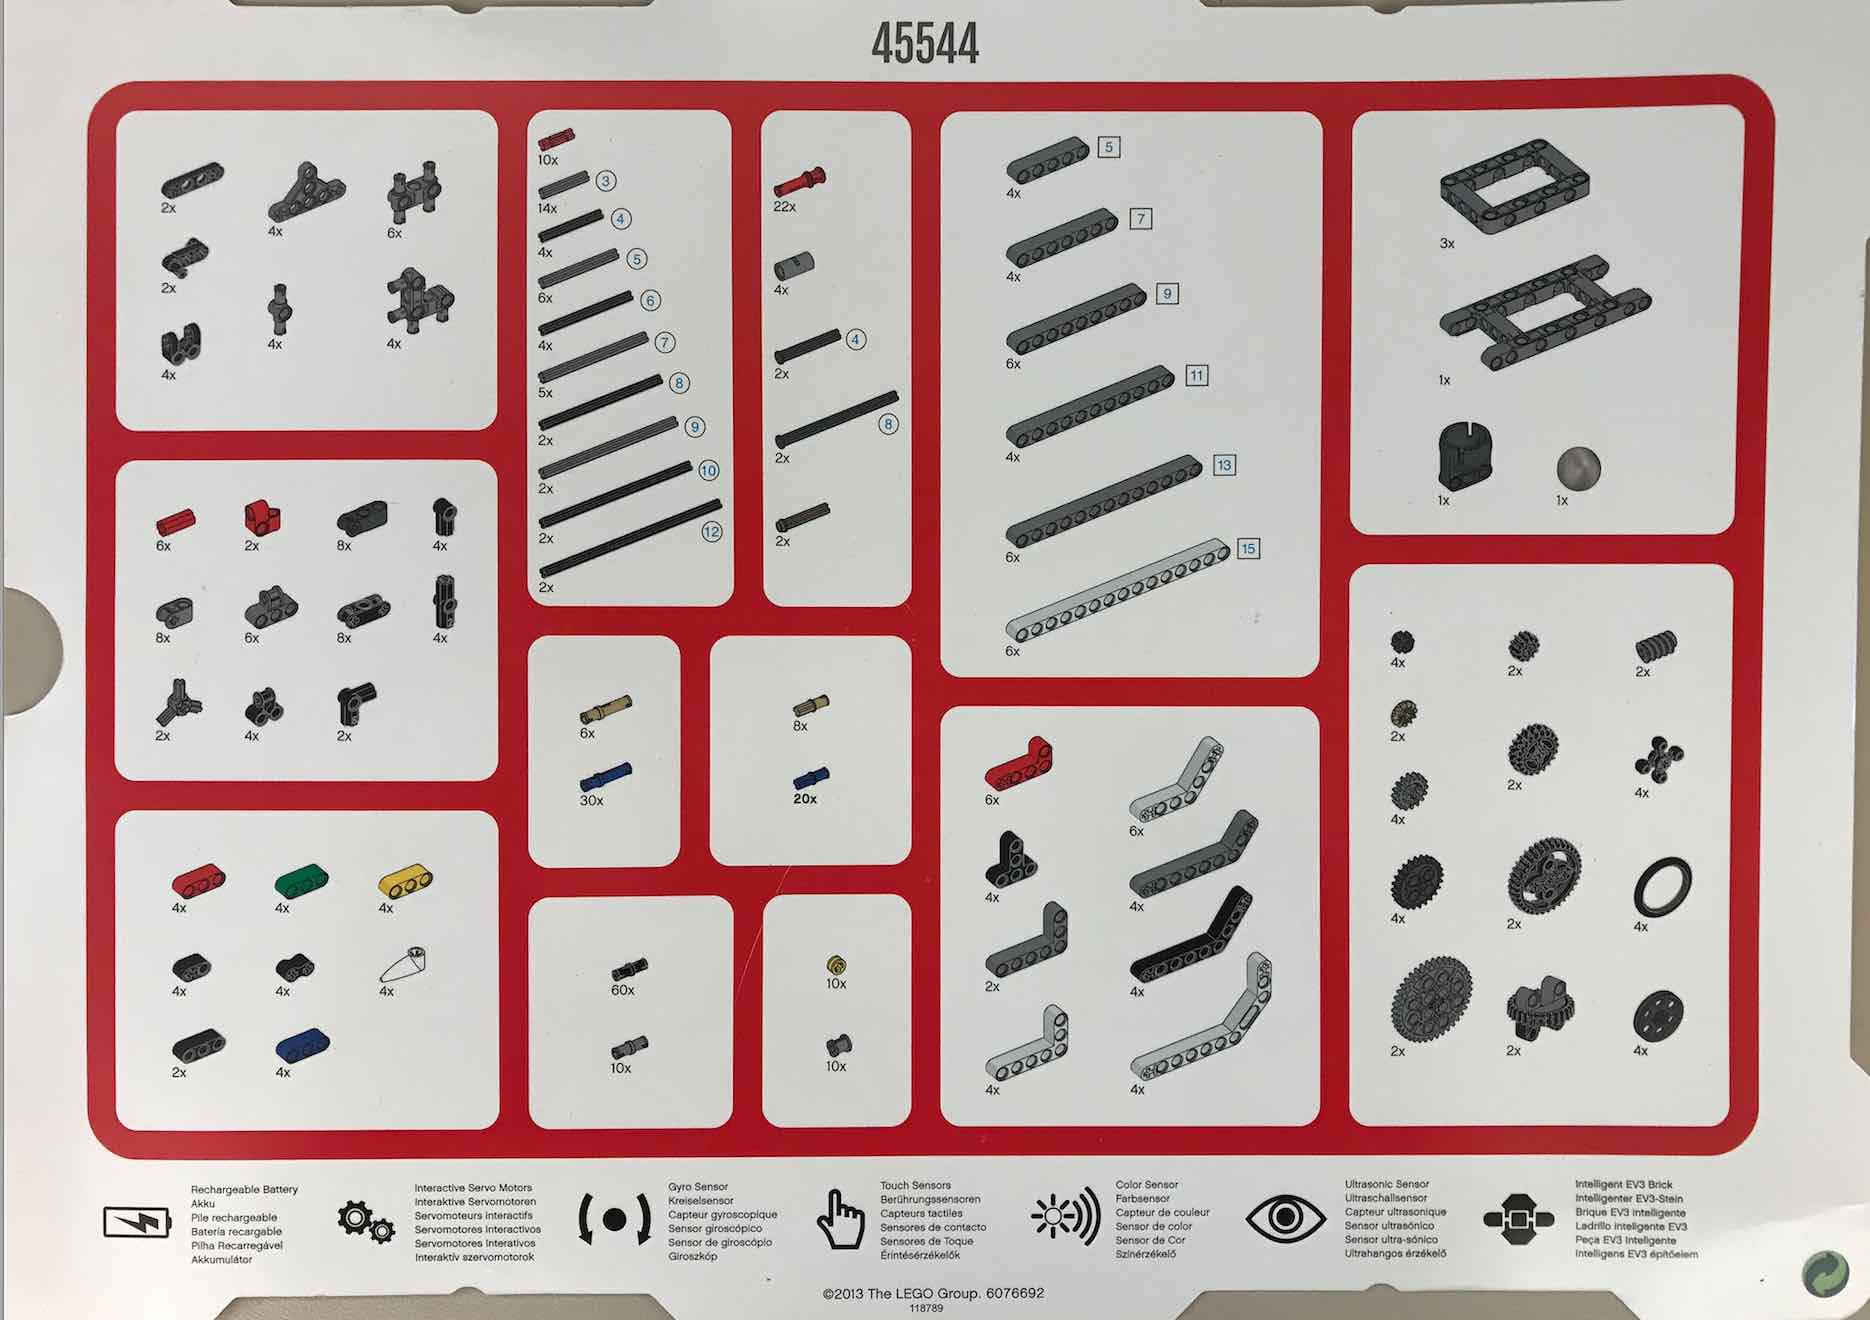
\includegraphics[angle=0, height=2.2in]{figures/kit1.jpg}
  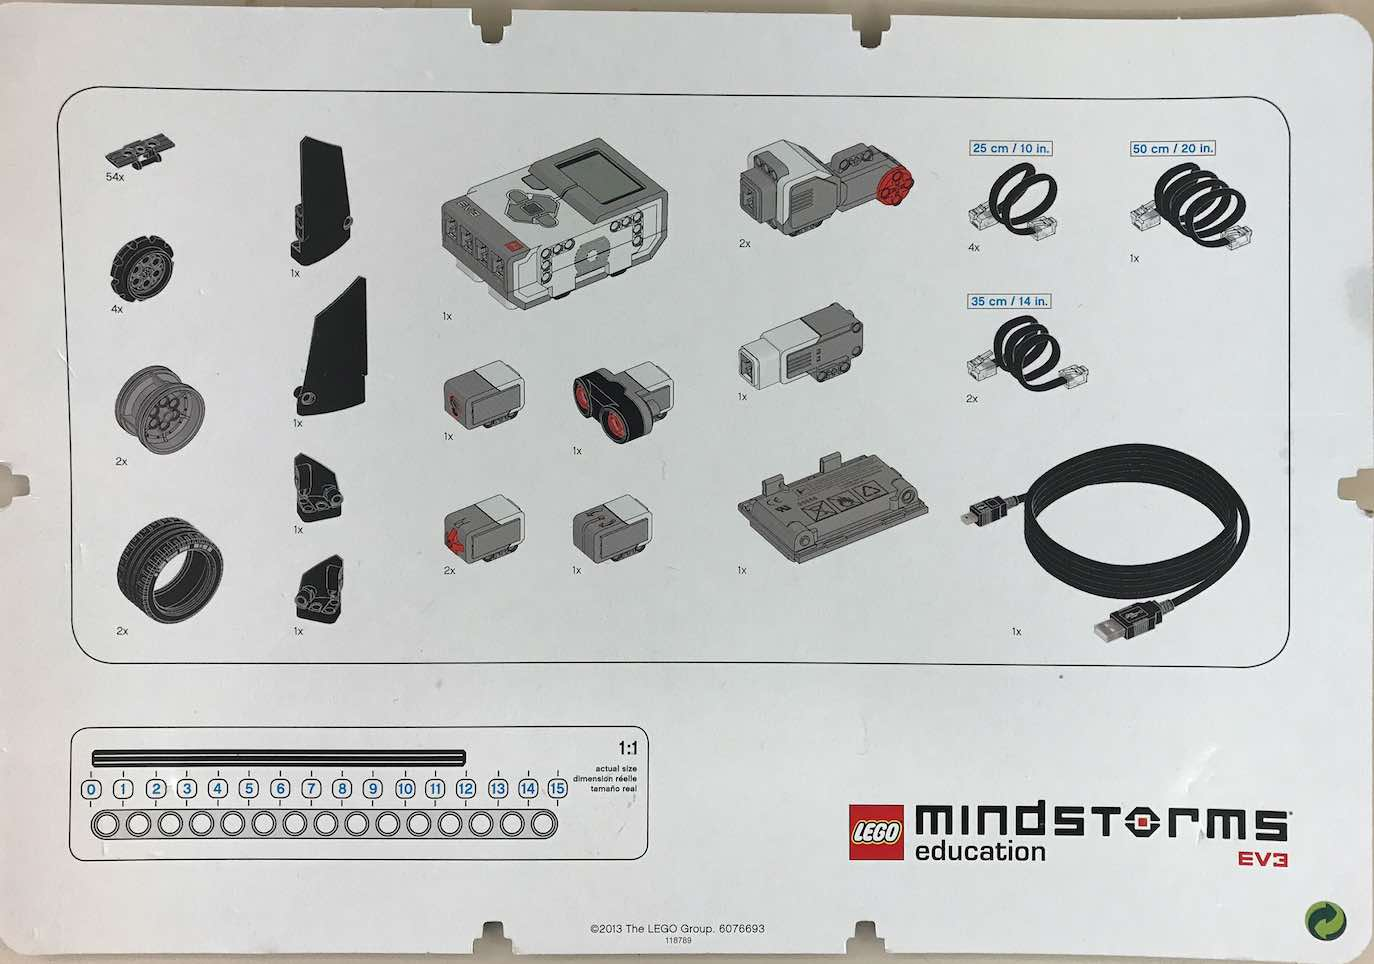
\includegraphics[angle=0, height=2.2in]{figures/kit2.jpg}
%  \includegraphics[angle=0, height=2.0in]{figures/lab4_parallel_park.pdf}
\end{center}
 \caption{This picture shows descriptions of components in the boxes.}
   \label{fig:kit1}
\end{figure}

% \begin{figure}[htbp]
%\begin{center}
%% 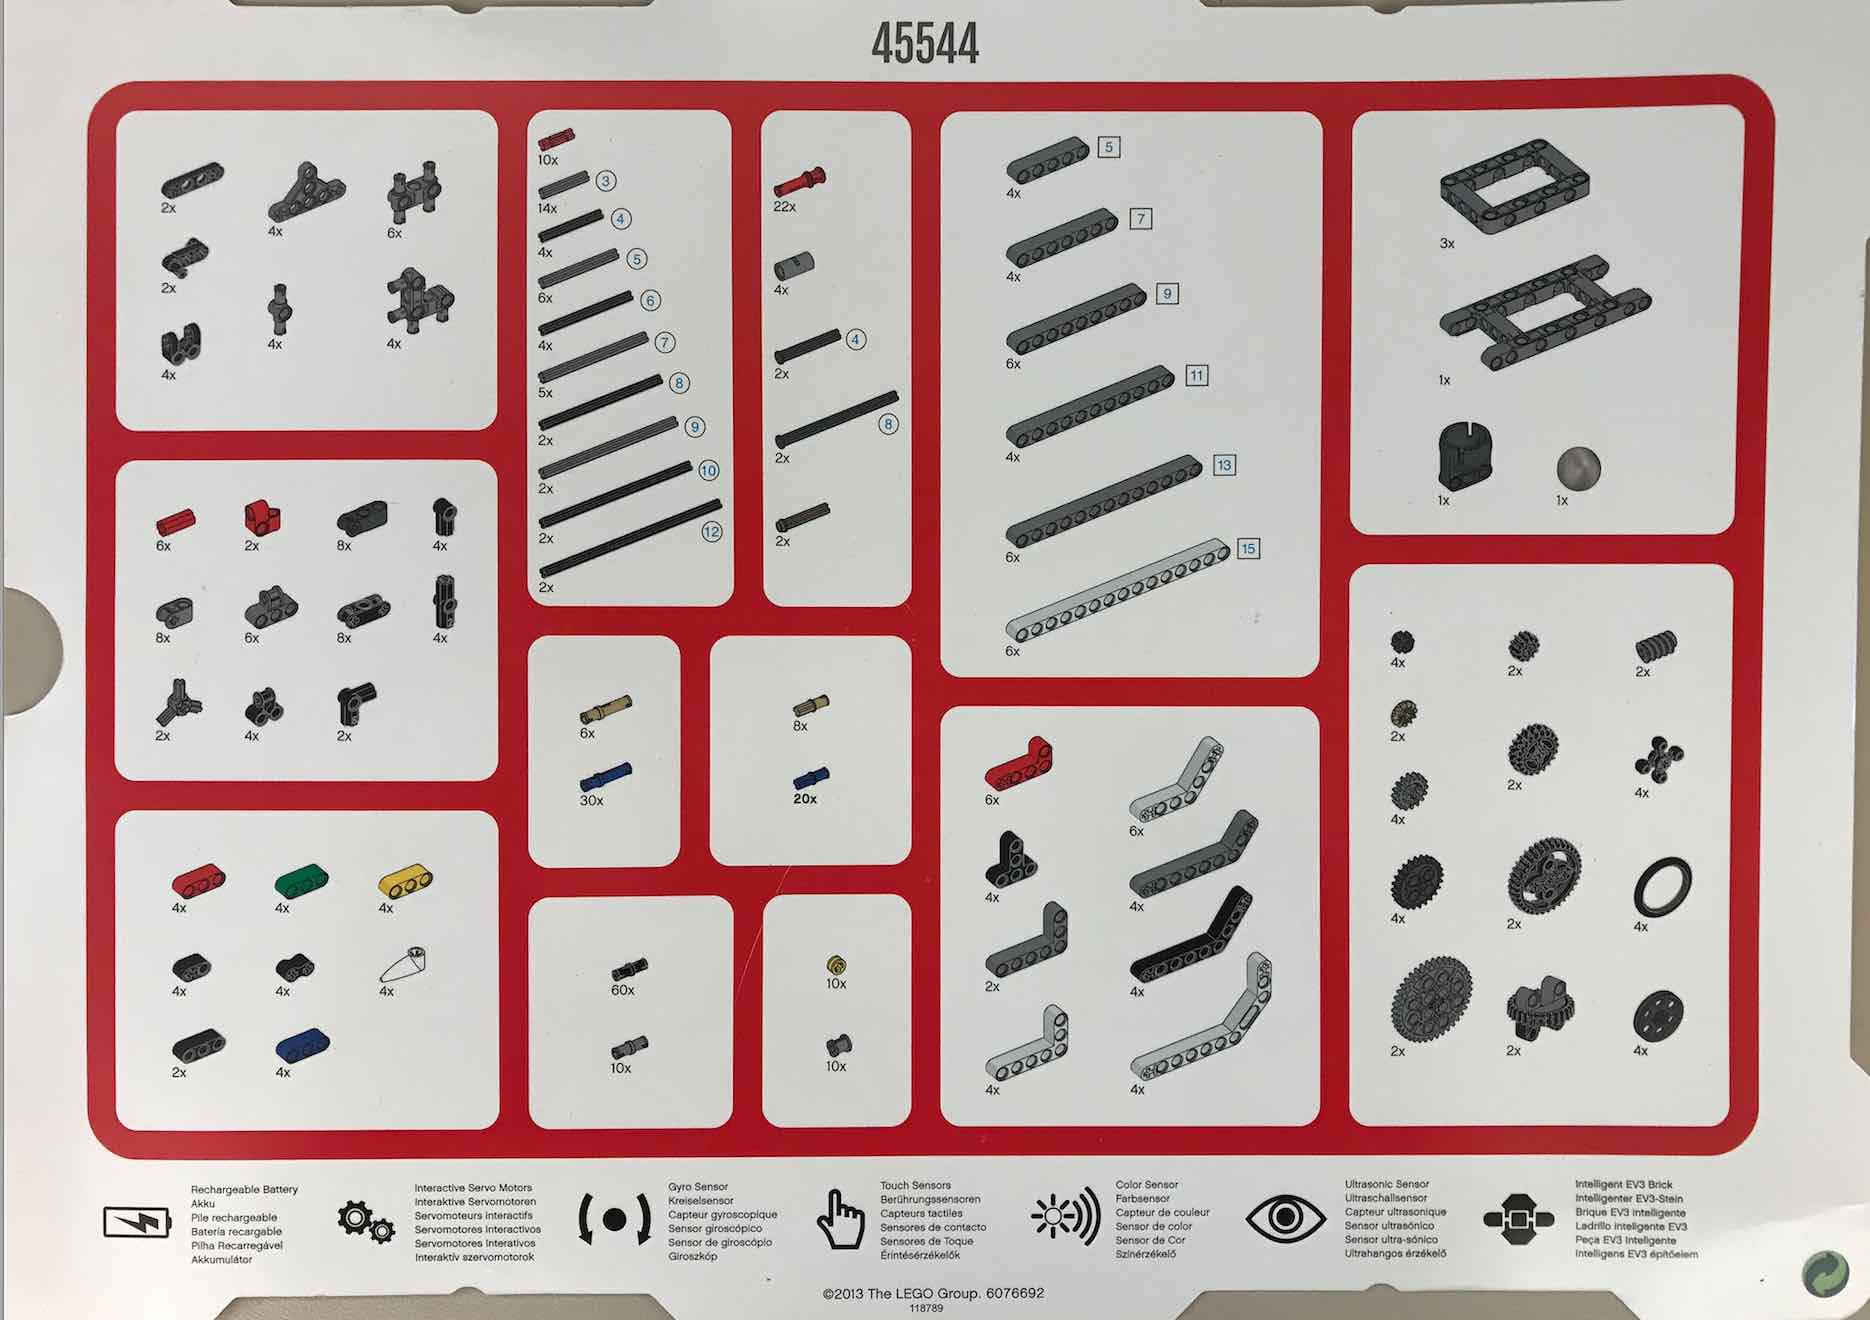
\includegraphics[angle=0, height=4in]{figures/kit1.jpg}
%  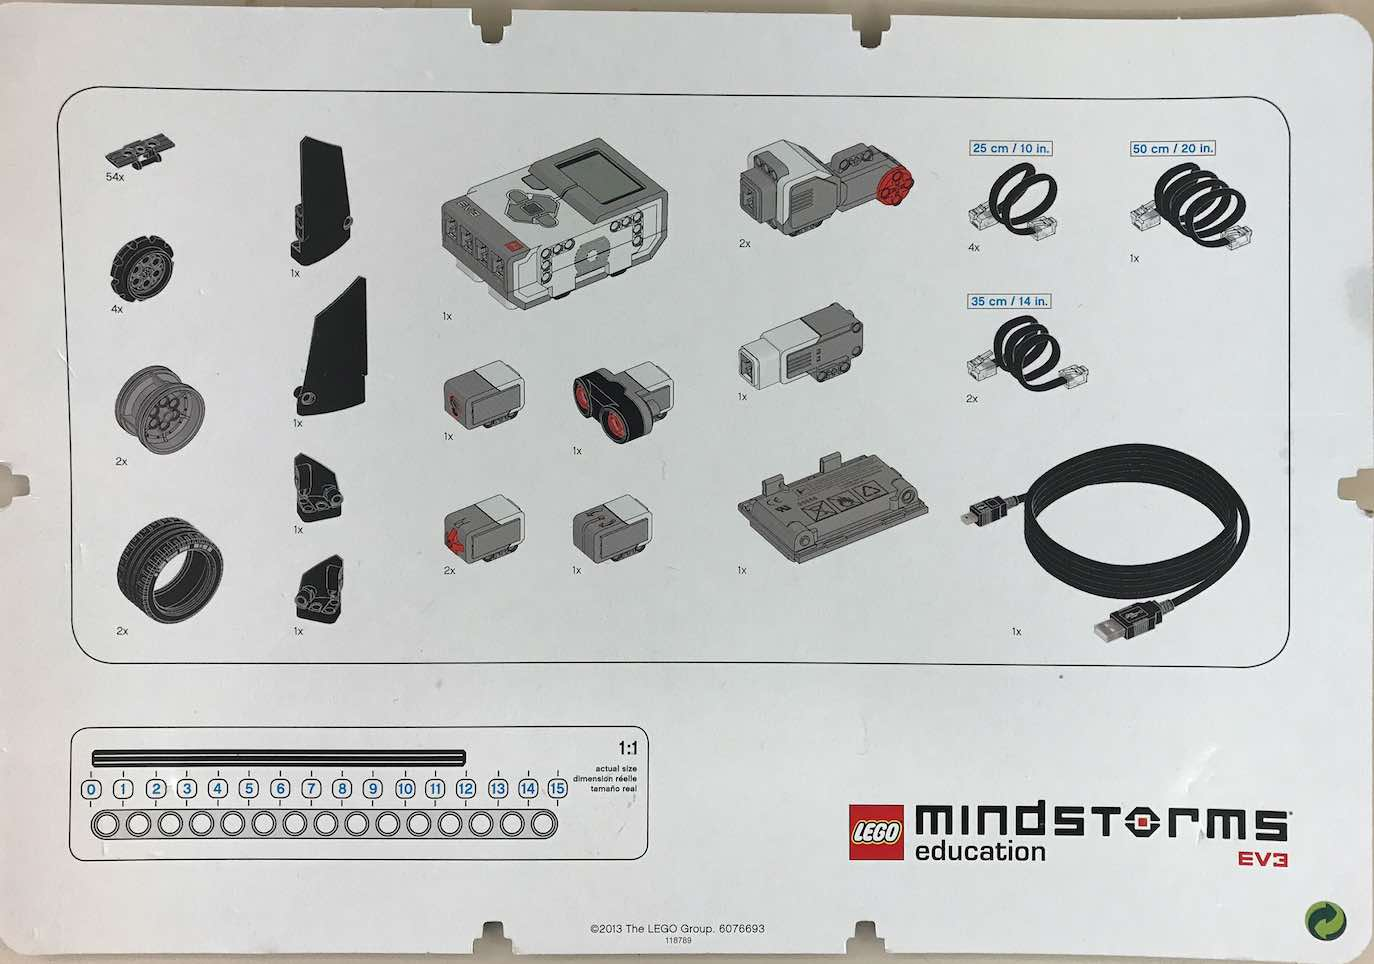
\includegraphics[angle=0, height=2.0in]{figures/kit2.jpg}
%%  \includegraphics[angle=0, height=2.0in]{figures/lab4_parallel_park.pdf}
%\end{center}
% \caption{This picture shows the computer (brick), sensors, and motors provided in the kit.}
%   \label{fig:kit2}
%\end{figure}


%\clearpage
%%%%%%%%%%%%%%%%%%%%%%%%%%%%%%%
\section*{Task 2: Introduction to brick programing}
%%The point of the homework is to help you get started with LEGO Mindstorms.
%\subsection*{Installation of LEGO software}
%Download the Mindstorms EV3 software and install it on your computer. Be sure to check the system requirement before you download and install the software.
%\bluehref{http://www.lego.com/en-us/mindstorms/downloads}{http://www.lego.com/en-us/mindstorms/downloads} 
%\\
%\\
%You might want to download the user guide and keep it handy \\
%Google search ``LEGO Mindstorms User Guide" (Size 7.8 MB)
%%\bluehref{http://tiny.cc/pranavb\_lego}{http://tiny.cc/pranavb\_lego} (Size 7.8 MB and links to the LEGO website)
%%\bluehref{http://cache.lego.com/r/www/r/mindstorms/-/media/franchises/mindstorms\%202014/downloads/user\%20guides/user\%20guide\%20lego\%20mindstorms\%20ev3\%2010\%20all\%20enus\%20(2).pdf?l.r2=-329554550}{http://cache.lego.com/r/www/r/mindstorms/-/media/franchises/mindstorms\%202014/downloads/user\%20guides/user\%20guide\%20lego\%20mindstorms\%20ev3\%2010\%20all\%20enus\%20(2).pdf?l.r2=-329554550}


%\subsection*{(a) Programming basics}
This video shows how to write a basic program that plays a sound using the brick.
\\
Video: 
\bluehref{https://youtu.be/81hctQt6Cp8}{https://youtu.be/81hctQt6Cp8} (Duration: 4 min 29 sec) \\
 \textcolor{magenta}{\bf Task 2: Follow the video and show your work to the teaching assistant.} 
 
 \section*{Task 3: Introduction to sensors}
 \subsection*{Programming the touch sensor}
This video shows you how to program a touch sensor \\
Video: 
\bluehref{https://youtu.be/QYHYA-\_d-8M}{https://youtu.be/QYHYA-\_d-8M} (Duration: 5 min 17 sec).\\
%Things to play with: 
%{\it Practise Exercise:} Find the other sensors in the kit. A list is provided above. Try to program each of them to understand their functionality. 
 \textcolor{magenta}{\bf Task 3a: Follow the video and show your work to the teaching assistant.}
%{\it Hint:} Read the manual. \bluehref{http://tiny.cc/pranavb\_lego}{http://tiny.cc/pranavb\_lego}

\subsection*{Programming color sensor}
Program the brick so that when the color sensor is shown one of the three colors; red, green, and blue; it is displayed on the brick. The TA will test the program by showing one of the three colors to the color sensor. Ask the TA to give you the color chart.
%The color chart for testing is here: \\ \bluehref{http://aux.coe.utsa.edu/~pab/info/lego/lego\_colors1.pdf}{http://aux.coe.utsa.edu/$\sim$pab/info/lego/lego\_colors1.pdf} %{\bf (10 points)} 
\\
 \textcolor{magenta}{\bf Task 3b: Call the TA once you are ready to demonstrate.}


\vspace{0.5cm}
\noindent \textcolor{red}{\bf\Large Day 1, Session 2: 1:00 PM -- 2:30 PM} 
\section*{Task 4: Introduction to motors}
\subsection*{Programming motors}
The video shows you how to make a motor move. At the end of this video you will be able to control the speed (magnitude and duration), and also control the angle of spin. \\ Video:
\bluehref{https://youtu.be/liKa\_I55ADM}{https://youtu.be/liKa\_I55ADM} (Duration: 4 min 58 sec). \\
 \textcolor{magenta}{\bf Task 4: Show this to the teaching assistant.}
%\\
%{\it Practise Exercise:} Can you find the two types of motors? Program any one to turn.
%{\it Hint:} Read the manual. \bluehref{http://tiny.cc/pranavb\_lego}{http://tiny.cc/pranavb\_lego}

\subsection*{Develop a mobile car}

\begin{enumerate}
\item Build the car shown here: \bluehref{https://youtu.be/HsLqiShzP0k}{https://youtu.be/HsLqiShzP0k} or use the booklet provided to you in the box (Duration 2 min 42 sec). 
 \item Program the car to move in the following fashion: (1) move straight for 2 seconds; (2) take a 90 turn to the right; (3) move straight for 2 seconds; (4) come to a stop. {\it HINT:} See the tutorial here.  \bluehref{https://youtu.be/8C01X72\_Xfk}{https://youtu.be/8C01X72\_Xfk} (Duration: 3 min 29 sec).
\end{enumerate}

\vspace{0.5cm}
\noindent \textcolor{red}{\bf\Large Day 1, Session 3: 3:00 PM -- 4:15 PM} 
\section*{Task 5: Car racing}
\subsection*{Reacting to sensor measurements}
The next task is a race that will be played by all teams together as shown in Fig.~\ref{fig:car_racing}. The goal is to program your car to move from start to end as shown. The moment the TA says ``Go" you will press a button on the brick initiating your car to move in a straight line towards the a red line as shown. The car which comes to a complete stop on the red line (color sensor on the car should be above the red line) first will be declared a winner. 
\begin{figure}[htbp]
\begin{center}
 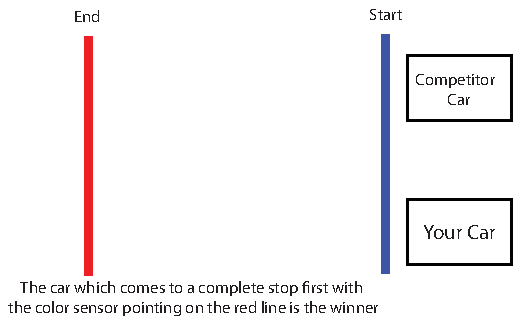
\includegraphics[angle=0, height=2.2in]{figures/car_race.pdf}
\end{center}
 \caption{Car racing conceptual diagram.}
   \label{fig:car_racing}
\end{figure}

\section*{Packing up}
Do not dis-assemble your car robot. You will need it tomorrow. Please ensure that your team's name and team member names are inside the box. Please return the box to the TA. 
%\begin{enumerate}
%\item Find the other sensors in the kit. A list is given above.
%\item Try to write at least one program per sensor to learn about how it works.
%\end{enumerate}

%\clearpage
%\section*{Task 3: Color Sensor}
%To get credit, you will need to demonstrate the following things to the teaching assistant. 


%HINT: Do not dis-assemble your car. You will be able to reuse the car in the next lab.

%\clearpage
%\includegraphics[scale=1]{figures/robot_trajectoryC.pdf}


%\section{Competition}
%There is no competition planned for this lab. Future labs will have a competition between teams.


%\subsection{Basic Soldering}
%Watch this youtube video first: \bluehref{https://www.youtube.com/watch?v=BLfXXRfRIzY}{https://www.youtube.com/watch?v=BLfXXRfRIzY}. \\
%Now solder two pieces of wire as shown towards the end of the video. Each person in the group should do this exercise and show it to the teaching assistant
%%%%%

%\subsection{Peer-Review}
%IMPORTANT: Ask the Lab Assistant to do a peer-review for effort before leaving the lab. It is your duty to remind the teaching assistant. Else, nobody will get credit for that particular lab.


\end{document}